\documentclass{article}
\usepackage[utf8]{inputenc}
\usepackage{listings}
\usepackage{color}
\usepackage{newunicodechar}
\usepackage{graphicx}
\usepackage{enumitem}
\usepackage{amsmath}
\usepackage{float}

% The offending character in the first argument
% and a hyphen in the second argument!
\newunicodechar{−}{-}

\begin{document}

\begin{titlepage}
    \begin{center}
        \vspace*{1cm}

        \large{Optimization Techniques (MA-526)}\\
        \Large{\textsc{\textbf{Variable Metric Method For Constrained Optimization}}}

        \vspace{1cm}

        \begin{table}[htbp]
    	\centering
    		\begin{tabular}{cc}
             Anandita & 14074001 \\
			 Ankit Saini & 14075008      \\        
             Ayush Shrivastava & 14075014\\
             Babloo Kumar & 14074005 \\
             Himanshu Agarwal & 14075031
            \end{tabular}
 		\end{table}

		\small{Senior Undergraduates\\
        Dept. of Computer Science and Engineering,\\
        Indian Institute of Technology (BHU) Varanasi}

		\vspace{1cm}

        \small{Under the guidance of}

        \vspace{0.5cm}

        \large{\textbf{Dr. Debdas Ghosh}}

        \vspace{0.5cm}

        \normalsize{\textbf{Assistant Professor\\
        Dept. of Mathematical Sciences,\\
        Indian Institute of Technology (BHU) Varanasi}}

        \vspace{1cm}

        
\includegraphics[width=0.4\textwidth]{iitbhu.png}

        \vspace{1cm}
    \end{center}
\end{titlepage}

\section{Introduction}

In the unconstrained optimization problems the desirable improved convergence rate of Newton’s method could be approached by using suitable update formulas to approximate the matrix of second derivatives. Thus, with the wisdom of hindsight, it is not surprising that, as first shown by Garcia- Palomares and Mangasarian [1], similar constructions can be applied to approximate the quadratic portion of our Lagrangian subproblems. The idea of approximating $\nabla^2L$ using quasi-Newton update formulas that only require differences of gradients of the Lagrangian function was further developed by Han [2, 3] and Powell [4, 5]. The basic variable metric strategy proceeds as follows.

\subsection{Description of the problem}
P :
\begin{equation*}
    \begin{aligned}
        & \text{Minimize}
        & & f(x) \\
        & \text{Subject to}
        & & h_k(x) = 0, \, k = 1, \ldots, K\\
        &&& g_j(x) \geq 0, \, j = 1, \ldots, J\\
    \end{aligned}
\end{equation*}


\subsection{Assumptions}
The following assumptions are taken into account:
\begin{itemize}
    \item $f$, $g_i$ and $h_j$ are differentiable.
    \item $g_i$ is continuous at $x^*$.
\end{itemize}

\section{Algorithm}

Given initial estimates $x^0$ , $u^0$ , $v^0$ and a symmetric positive-definite matrix $H^0$.\newline

\textbf{Step 1. }Solve the problem
\begin{equation*}
    \begin{aligned}
        & \text{Minimize}
        & & \nabla f(x^{(t)})^Td + \frac{1}{2}d^T\textbf{H}^{(t)}d \\
        & \text{Subject to}
        & & h_k(x^{(t)}) + \nabla h_k(x^{(t)})^Td = 0, \, k = 1, \ldots, K\\
        &&& g_j(x^{(t)}) + \nabla g_j(x^{(t)})^Td \geq 0, \, j = 1, \ldots, J\\
    \end{aligned}
\end{equation*}

\textbf{Step 2. }Select the step size $\alpha$ along $d^{(t)}$ and set $x^{(t+1)} = x^{(t)} + \alpha d^{(t)}$.

\textbf{Step 3. }Check for convergence.

\textbf{Step 4. }Update $\textbf{H}^{(t)}$ using the gradient difference
\[\nabla_xL(x^{(t+1)}, u^{(t+1)}, v^{(t+1)}) - \nabla_xL(x^{(t)}, u^{(t+1)}, v^{(t+1)})\]
in such a way that $\textbf{H}^{(t+1)}$ remains positive definite.\newline

The key choices in the above procedure involve the update formula for $\textbf{H}^{(t)}$ and the manner of selecting $\alpha$ . Han [1, 2] considered the use of several well-known update formulas, particularly DFP. He also showed [1] that if the initial point is sufficiently close, then convergence will be achieved at a superlinear rate without a step-size procedure or line search by setting $\alpha = 1$. However, to assure convergence from arbitrary points, a line search is required. Specifically, Han [2] recommends the use of the penalty function
\[P(x, R) = f(x) + R\{\sum_{k=1}^{K} |h_k(x)| - \sum_{j=1}^{J} min(0,g_j(x))\}\]
to select $\alpha^*$ so that
\[P(x(\alpha^*)) = \min_{0\leq\alpha\leq\delta} P(x^{(t)} + \alpha d^{(t)}), R)\]
where R and $\delta$ are suitably selected positive numbers.\par
Powell [4], on the other hand, suggests the use of the BFGS formula together with a conservative check that ensures that $\textbf{H}^{(t)}$ remains positive definite. Thus, if
\[z = x^{(t+1)} - x^{(t)}\]
and
\[y = \nabla_xL(x^{(t+1)}, u^{(t+1)}, v^{(t+1)}) - \nabla_xL(x^{(t)}, u^{(t+1)}, v^{(t+1)})\]
Then define
\[
    \theta =
    \begin{cases}
        1 & \text{if $z^Ty \geq 0.2z^T\textbf{H}^{(t)}z$}\\
        \frac{0.8z^T\textbf{H}^{(t)}z}{z^T\textbf{H}^{(t)}z - z^Ty} & \text{otherwise}
    \end{cases}
\]
and calculate
\[w = \theta y + (1-\theta) \textbf{H}^{(t)}z\]
Finally, this value of $w$ is used in the BFGS updating formula,
\[\textbf{H}^{(t+1)} = \textbf{H}^{(t)}-\frac{\textbf{H}^{(t)}zz^T\textbf{H}^{(t)}}{z^T\textbf{H}^{(t)}z^T}+\frac{ww^T}{z^Tw} \]

Note that the numerical value 0.2 is selected empirically and that the normal BFGS update is usually stated in terms of $y$ rather than $w$.\par
On the basis of empirical testing, Powell [5] proposed that the step-size procedure be carried out using the penalty function
\[P(x, \mu, \sigma) = f(x) + \sum_{k=1}^{K} \mu_k|h_k(x)| - \sum_{j=1}^{J} \sigma_j min(0,g_j(x))\]
where for the first iteration
\[\mu_k = |v_k|, \sigma_j = |u_j|\]
and for all subsequent iterations t
\[\mu_k^{(t)} = max(|v_k^{(t)}|,\frac{1}{2}(\mu_k^{(t-1)} + |v_k^{(t)}|))\]
\[\sigma_j^{(t)} = max(|u_j^{(t)}|,\frac{1}{2}(\sigma_j^{(t-1)} + |u_j^{(t)}|))\]
The line search could be carried out by selecting the largest value of $\alpha , 0 \leq \alpha \leq1$, such that
\[P(x(\alpha)) < P(x(0))\]
However, Powell [5] prefers the use of quadratic interpolation to generate a sequence of values of $\alpha_k$ until the more conservative condition
\[P(x(\alpha_k)) \leq P(x(0)) + 0.1\alpha_k\frac{dP}{d\alpha}(x(0))\]
is met. It is interesting to note, however, that examples have been found for which the use of Powell’s heuristics can lead to failure to converge [6]. Further refinements of the step-size procedure have been reported [7], but these details are beyond the scope of the present treatment.\par
%We illustrate the use of a variant of the constrained variable metric (CVM) method using update (10.11), penalty function (10.12), and a simple quadratic interpolation-based step-size procedure.


\section{Implementation}

The code was written in Python language, using Numpy, Scipy and Matplotlib libraries.\\ \\
\textbf{Environment Setup}

\begin{list}{•}{ }
\item Python 2.7.14
\item matplotlib 2.1.0
\item numpy 1.13.3
\item scipy 1.0.0
\end{list}

The code can be found in Appendix in Section 6.

\section{Evalution and Results}

\subsection*{Example 1}
\subsubsection*{Problem Statement}
\begin{equation*}
    \begin{aligned}
        & \text{Minimize}
        & & f(x) = 6x_1x_2^{-1} + x_2x_1^{-1} \\
        & \text{Subject to}
        & & h(x) = x_1x_2 - 2 = 0\\
        &&& g(x) = x_1 + x_2 -1 \geq 0\\
        & \text{Initialisation}
        & & x^0 = (2,1) , H^0 = I
    \end{aligned}
\end{equation*}
\subsubsection*{Results}
\begin{table}[H]
\centering
\caption{Values of $\mathbf{x_1}$, $\mathbf{x_2}$ and $\mathbf{f(x)}$ after each iteration}
\label{my-label1}
\begin{tabular}{|l|l|l|l|}\hline
\textbf{Iteration} & $\mathbf{x_1}$ & $\mathbf{x_2}$ & $\mathbf{f(x)}$ \\ \hline
1 & 1.450  & 1.274 & 7.43474 \\ \hline
2 & 1.350  & 1.363 & 6.68951 \\ \hline
3 & 1.343  & 1.371 & 6.63966 \\ \hline
4 & 1.399  & 1.428 & 6.60628 \\ \hline
5 & 1.397  & 1.430 & 6.59488 \\ \hline
6 & 1.394  & 1.434 & 6.57176 \\ \hline
7 & 1.389  & 1.439 & 6.53692 \\ \hline
8 & 1.378  & 1.451 & 6.46293 \\ \hline
9 & 1.364  & 1.465 & 6.37562 \\ \hline
10 & 1.347 & 1.483 & 6.26813 \\ \hline
11 & 1.328 & 1.504 & 6.14924 \\ \hline
12 & 1.312 & 1.524 & 6.05084 \\ \hline
13 & 1.286 & 1.553 & 5.90833 \\ \hline
14 & 1.265 & 1.579 & 5.79306 \\ \hline
15 & 1.240 & 1.611 & 5.66654 \\ \hline
16 & 1.220 & 1.638 & 5.56931 \\ \hline
17 & 1.194 & 1.673 & 5.45614 \\ \hline
18 & 1.174 & 1.702 & 5.37209 \\ \hline
19 & 1.145 & 1.744 & 5.27006 \\ \hline
20 & 1.124 & 1.777 & 5.20153 \\ \hline
21 & 1.094 & 1.826 & 5.12007 \\ \hline
22 & 1.074 & 1.861 & 5.07568 \\ \hline
23 & 1.046 & 1.909 & 5.03189 \\ \hline
24 & 1.031 & 1.938 & 5.01439 \\ \hline
25 & 1.014 & 1.971 & 5.00332 \\ \hline
26 & 1.006 & 1.986 & 5.00074 \\ \hline
27 & \textbf{1.001} & \textbf{1.996} & \textbf{5.00007} \\ \hline
\end{tabular}
\end{table}

\subsubsection*{Graph}

\begin{figure}[H]
\centering
    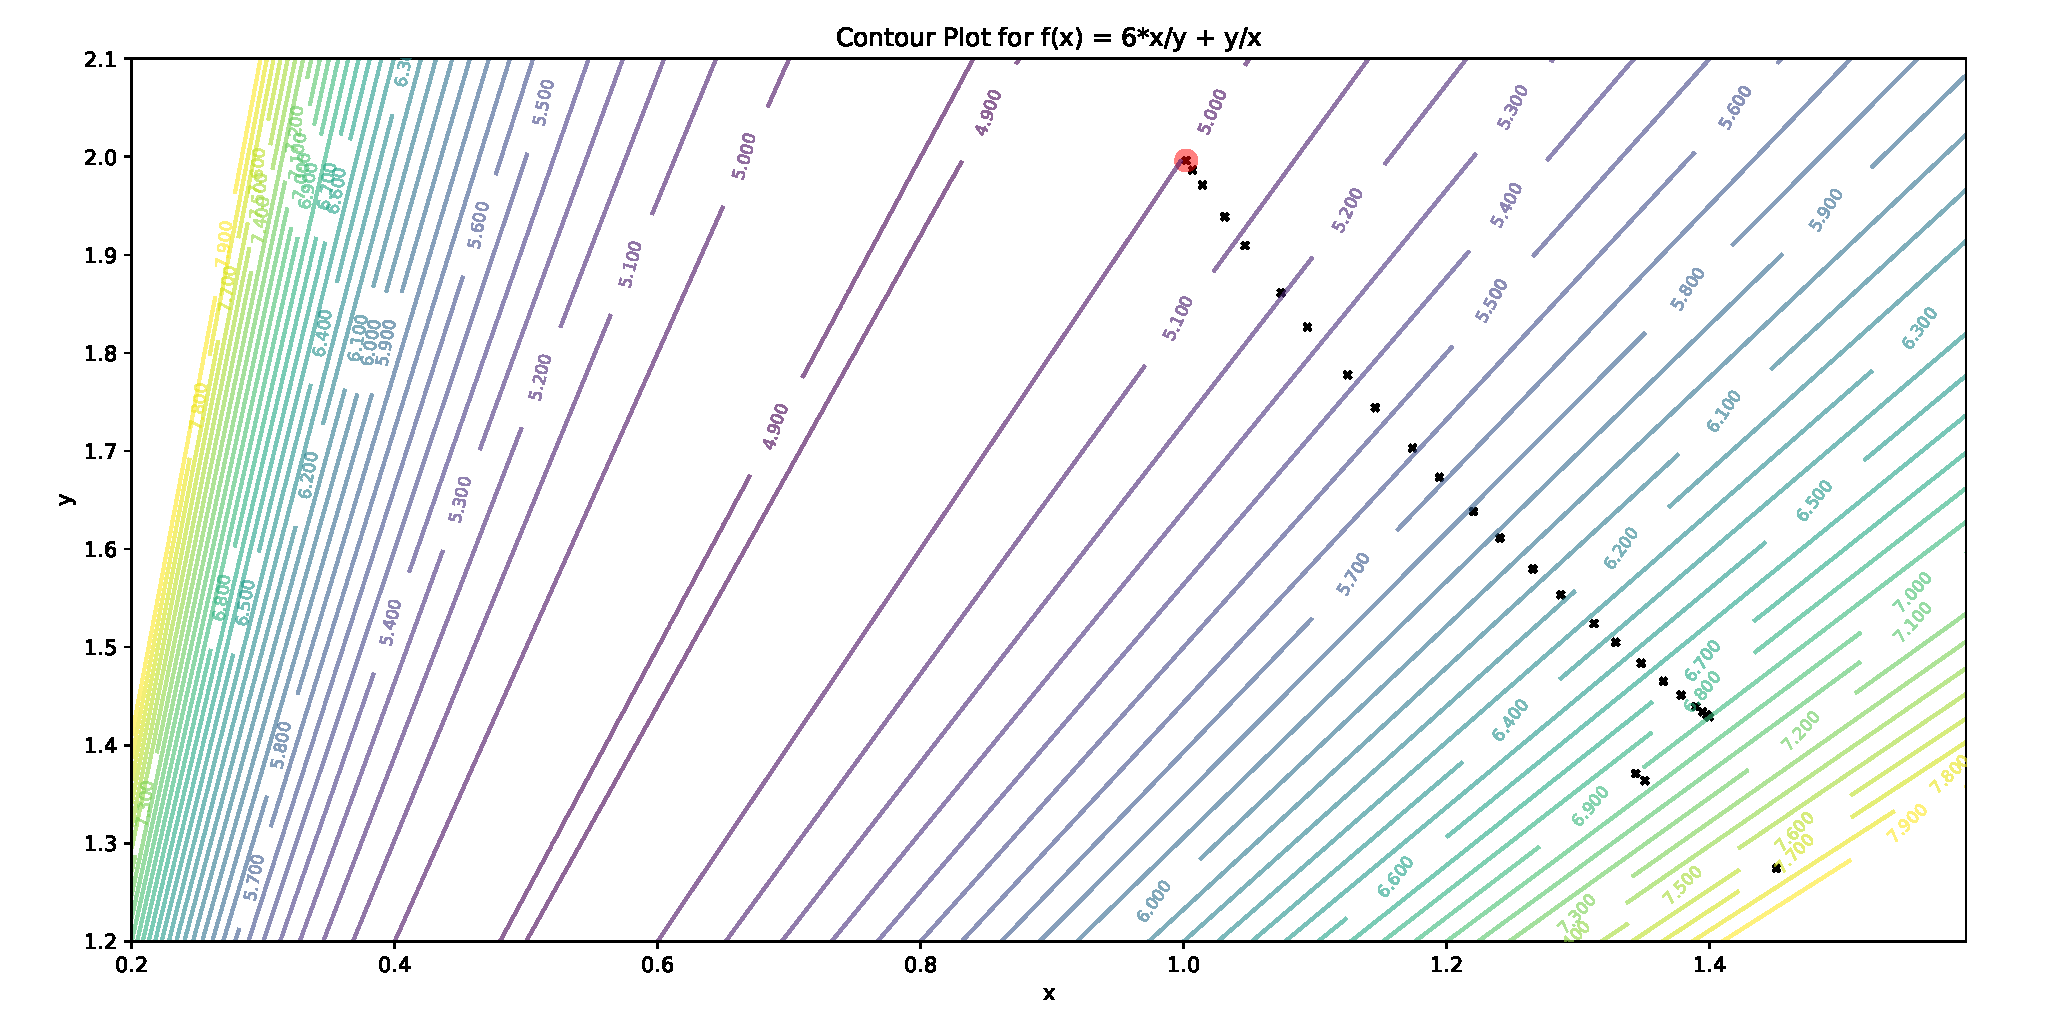
\includegraphics[width=450px]{graph1.pdf}
%\caption{ }
\label{fig:acc1}
\end{figure}

\subsection*{Example 2}

\subsubsection*{Problem Statement}

\begin{equation*}
    \begin{aligned}
        & \text{Minimize}
        & & f(x) = 3x_1^{2} - 4x_2 \\
        & \text{Subject to}
        & & h(x) = 2x_1 + x_2 - 4 = 0\\
        &&& g(x) = 37 - x_1^2 - x_2^2 \geq 0\\
        & \text{Initialisation}
        & & x^0 = (50,50) , H^0 = I
    \end{aligned}
\end{equation*}
\subsubsection*{Results}
\begin{table}[H]
\centering
\caption{Values of $\mathbf{x_1}$, $\mathbf{x_2}$ and $\mathbf{f(x)}$ after each iteration}
\label{my-label1}
\begin{tabular}{|l|l|l|l|}\hline
\textbf{Iteration} & $\mathbf{x_1}$ & $\mathbf{x_2}$ & $\mathbf{f(x)}$ \\ \hline

1 &  -18.005 & 82.983 & 640.69981 \\ \hline
2 &  -17.892 & 39.785 & 801.31495 \\ \hline
3 &   -6.114 & 16.228 &  47.23222 \\ \hline
4 &   -1.326 &  6.653 & -21.33320 \\ \hline
5 &   -1.018 &  6.036 & -21.03549 \\ \hline
6 & \textbf{-1.000} & \textbf{6.000} & \textbf{-21.00012} \\ \hline
\end{tabular}
\end{table}

\subsubsection*{Graph}

\begin{figure}[H]
\centering
    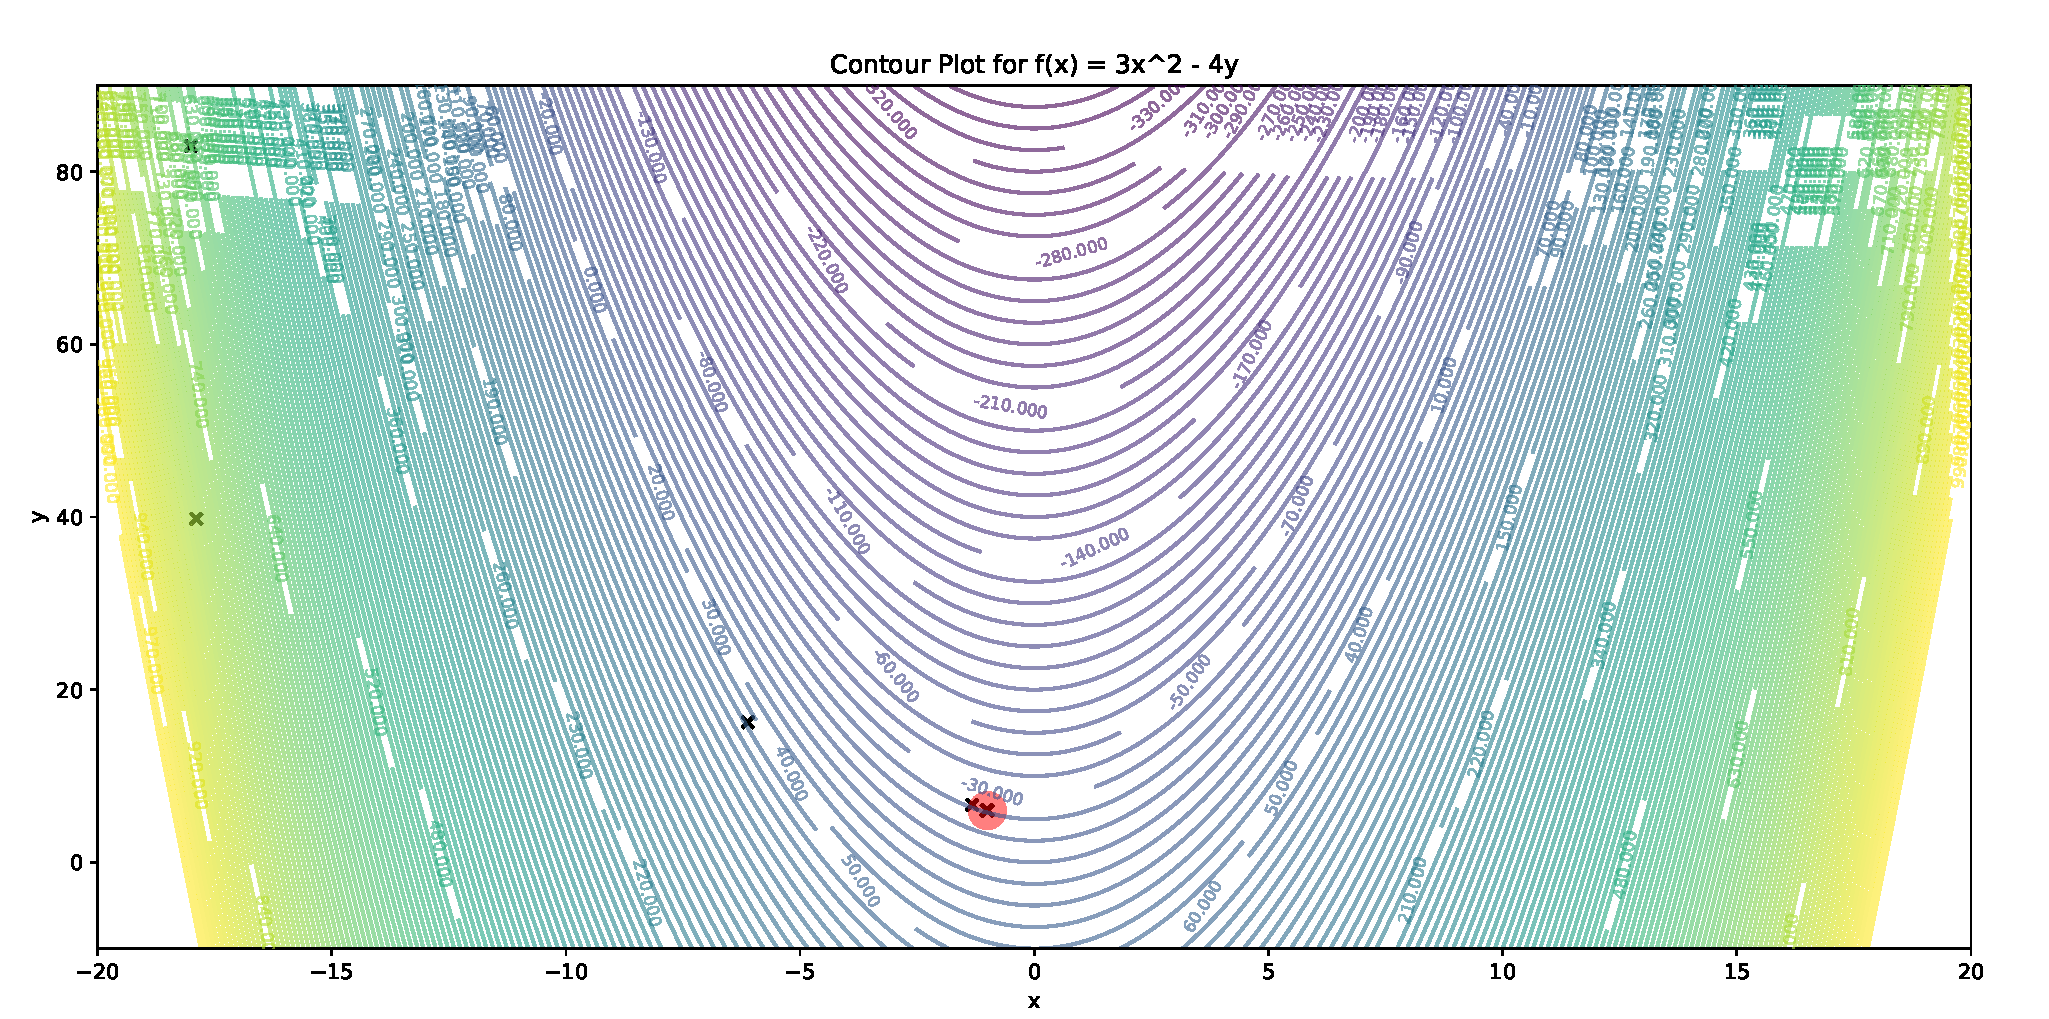
\includegraphics[width=450px]{graph2.pdf}
%\caption{ }
\label{fig:acc2}
\end{figure}


%\section{Conclusion}
%
%It should be emphasized that the available convergence results assume that the penalty function parameters remain unchanged and that exact line searches are used. Powell’s modifications and the use of approximate searches thus amount to useful heuristics justified solely by numerical experimentation. It is of interest that as reported by Bartholomew-Biggs [8], a code implementing this approach (OPRQ) has been quite successful in solving a number of practical problems, including one with as many as 79 variables and 190 constraints. This gives further support to the still sparse but growing body of empirical evidence suggesting the power of CVM approaches

\section{References}

[1] Garcia-Palomares, U. M., and O. L. Mangasarian, ‘‘Superlinearly Convergent
Quasi-Newton Algorithms for Nonlinearly Constrained Optimization Problem,’’
Math. Prog., 11, 1–13 (1976).
\newline\newline
[2] Han, S. P., ‘‘Superlinearly Convergent Variable Metric Algorithms for General Nonlinear Programming Problems,’’ Math. Prog., 11, 263–282 (1976).
\newline\newline
[3] Han, S. P., ‘‘A Globally Convergent Method for Nonlinear Programming,’’ J. Opt. Theory Appl. 22, 297–309 (1977).
\newline\newline
[4] Powell, M. J. D., ‘‘A Fast Algorithm for Nonlinearly Constrained Optimization Calculations,’’ in Numerical Analysis, Dundee 1977 (G. A. Watson, Ed.), Lecture Notes in Mathematics No. 630, Springer-Verlag, New York, 1978.
\newline\newline
[5] Powell, M. J. D., ‘‘Algorithms for Nonlinear Functions that Use Lagrangian Functions,’’ Math. Prog., 14, 224–248 (1978)
\newline\newline
[6] Chamberlain, R. M., ‘‘Some Examples of Cycling in Variable Metric Methods for Constrained Minimization,’’ Math. Prog., 16, 378–383 (1979).
\newline \newline
[7] Mayne, D. Q., ‘‘On the Use of Exact Penalty Functions to Determine Step Length in Optimization Algorithms,’’ in Numerical Analysis, Dundee, 1979 (G. A. Watson, Ed.), Lecture Notes in Mathematics No. 773, Springer-Verlag, New York, 1980.
\newline \newline
[8] Bartholemew-Biggs, M. C., ‘‘Recursive Quadratic Programming Based on Penalty Functions for Constrained Minimization,’’ in Nonlinear Optimization: Theory and Algorithms (L. C. W. Dixon, E. Spedicato, and G. P. Szego, Eds.), Birkhauser, Boston, 1980.

\section{Appendix}
In this section we present our implementation of the Mental Poker using socket programming in Python 3.

%New colors defined below
\definecolor{codegreen}{rgb}{0,0.6,0}
\definecolor{codegray}{rgb}{0.5,0.5,0.5}
\definecolor{codepurple}{rgb}{0.58,0,0.82}
\definecolor{backcolour}{rgb}{0.95,0.95,0.92}

%Code listing style named "mystyle"
\lstdefinestyle{mystyle}{
  backgroundcolor=\color{backcolour},   commentstyle=\color{codegreen},
  keywordstyle=\color{magenta},
  numberstyle=\tiny\color{codegray},
  stringstyle=\color{codepurple},
  basicstyle=\footnotesize,
  breakatwhitespace=false,
  breaklines=true,
  captionpos=b,
  keepspaces=true,
  numbers=left,
  numbersep=5pt,
  showspaces=false,
  showstringspaces=false,
  showtabs=false,
  tabsize=2
}

%"mystyle" code listing set
\lstset{style=mystyle}

%Python code highlighting
\begin{lstlisting}[language=Python, caption=main.py]
import numpy as np
from scipy import optimize
from sympy import *
import matplotlib.pyplot as plt
from mpl_toolkits.mplot3d import Axes3D
from matplotlib import cm

x_values = []

def list_to_array(x):
    return np.array(x, dtype = np.float64).reshape(2, 1)

def calculate_function_value(fx, xvars, xcurr):
    return fx.subs(zip(xvars,xcurr))

def find_dk(curr_fx, curr_hx, curr_gx, curr_grad_fx, curr_grad_hx, curr_grad_gx, H):
    curr_grad_fx = list_to_array(curr_grad_fx)
    curr_grad_gx = list_to_array(curr_grad_gx)
    curr_grad_hx = list_to_array(curr_grad_hx)

    new_hx = lambda d : curr_hx + np.matmul(np.transpose(curr_grad_hx), list_to_array(d))
    new_gx = lambda d : curr_gx + np.matmul(np.transpose(curr_grad_gx), list_to_array(d))
    objective = lambda d :  np.matmul(np.transpose(curr_grad_fx), list_to_array(d)) + (np.matmul(np.transpose(list_to_array(d)), np.matmul(H, list_to_array(d))))/2

    constraints = ({'type': 'eq', 'fun': new_hx},
                   {'type': 'ineq', 'fun': new_gx})

    result = optimize.minimize(objective, [1.0, 1.0], constraints = constraints)
    return result.x

def find_lagrange_multipliers(curr_fx, curr_hx, curr_gx, curr_grad_fx, curr_grad_hx, curr_grad_gx, H, d):
    A = np.array( ( [ curr_grad_hx[0], curr_grad_gx[0] ], [ curr_grad_hx[1], curr_grad_gx[1]] ), dtype = np.float64)
    B = np.array( [ curr_grad_fx[0] + H[0][0]*d[0] + (H[0][1] + H[1][0])*d[1] , curr_grad_fx[1] + H[1][1]*d[1] + (H[0][1] + H[1][0])*d[0] ], dtype = np.float64 ).reshape(2,1)
    A_inverse = np.linalg.inv(A)
    X = np.matmul(A_inverse,B)
    return X[0][0], X[1][0]

def calculate_mu_sigma(k, u, v, mu_k_1, sigma_k_1):
    if k==1:
        mu_k = abs(v)
        sigma_k = abs(u)
    else:
        mu_k = max(abs(v),(mu_k_1+abs(v))/2)
        sigma_k = max(abs(u), (sigma_k_1+abs(u))/2)
    return mu_k, sigma_k


def minimize_alpha_through_penalty_function(fx, hx, gx, mu_k, sigma_k, x_k_1, d_k):
    alpha = symbols('alpha')
    Px = fx + mu_k*abs(hx) - sigma_k*Min(0, gx)
    P_alpha = Px.subs([(x1,x_k_1[0]+alpha*d_k[0]), (x2,x_k_1[1]+alpha*d_k[1])])
    call_P = lambda alpha : P_alpha.subs([('alpha',alpha)])
    constraints = ({'type': 'ineq', 'fun': lambda alpha: alpha},
                   {'type': 'ineq', 'fun': lambda alpha: 1-alpha})
    alpha_k = optimize.minimize(call_P, 0, constraints = constraints).x
    return alpha_k

def calculate_y(grad_L, x_k, x_k_1):
    return np.array([i.subs([(x1,x_k[0]),(x2,x_k[1])]) for i in grad_L]) - np.array([i.subs([(x1,x_k_1[0]),(x2,x_k_1[1])]) for i in grad_L])

def calculate_theta(z, y, H):
    z = z.reshape(2,1).astype(np.float64)
    y = y.reshape(2,1).astype(np.float64)
    a1 = np.matmul(np.transpose(z),y)
    a2 = 0.2*np.matmul(np.transpose(z), np.matmul(H,z))
    if(a1>=a2):
        return np.array([[1]])
    else:
        return (0.8*np.matmul(np.transpose(z), np.matmul(H,z)))/(np.matmul(np.transpose(z), np.matmul(H,z)) - np.matmul(np.transpose(z),y))

def calculate_w(theta, H, z, y):
    z = z.reshape(2,1).astype(np.float64)
    y = y.reshape(2,1).astype(np.float64)
    theta = theta[0][0]
    return theta*y + (1-theta)*np.matmul(H,z)

def updateH(H, z, w):
    z = z.reshape(2,1).astype(np.float64)
    w = w.reshape(2,1).astype(np.float64)
    a1 = np.matmul(H , np.matmul(z, np.matmul(np.transpose(z) , H ))) / np.matmul(np.transpose(z) , np.matmul(H, z) )
    a2 = np.matmul(w, np.transpose(w)) / np.matmul(np.transpose(z), w)
    return H - a1 + a2

def constrained_variable_metric_method(fx, hx, gx, x_0, H_0, xvars, no_of_iterations):
    d1, d2 = symbols('d1 d2')
    dvars = [d1, d2]

    grad_fx = np.array([ diff(fx, x) for x in xvars ])
    grad_hx = np.array([ diff(hx, x) for x in xvars ])
    grad_gx = np.array([ diff(gx, x) for x in xvars ])

    x_k_1 = x_0
    H_k_1 = H_0

    mu_k_1 = 0
    sigma_k_1 = 0

    for k in range(1,no_of_iterations+1):

        xcurr = x_k_1
        H_k = H_k_1

        curr_fx = np.array([ fx.subs(zip(xvars,xcurr)) ])
        curr_hx = np.array([ hx.subs(zip(xvars,xcurr)) ])
        curr_gx = np.array([ gx.subs(zip(xvars,xcurr)) ])

        curr_grad_fx = np.array([ dfx.subs(zip(xvars,xcurr)) for dfx in grad_fx ])
        curr_grad_hx = np.array([ dhx.subs(zip(xvars,xcurr)) for dhx in grad_hx ])
        curr_grad_gx = np.array([ dgx.subs(zip(xvars,xcurr)) for dgx in grad_gx ])

        d_k = find_dk(curr_fx, curr_hx, curr_gx, curr_grad_fx, curr_grad_hx, curr_grad_gx, H_k)

        v, u = find_lagrange_multipliers(curr_fx, curr_hx, curr_gx, curr_grad_fx, curr_grad_hx, curr_grad_gx, H_k, d_k)

        mu_k, sigma_k = calculate_mu_sigma(k, u, v, mu_k_1, sigma_k_1)

        alpha_k = minimize_alpha_through_penalty_function(fx, hx, gx, mu_k, sigma_k, x_k_1, d_k)

        x_k = x_k_1 + alpha_k*d_k.reshape(2)

        z = x_k - x_k_1

        grad_L = grad_fx - v*grad_hx - u*grad_gx

        y = calculate_y(grad_L, x_k, x_k_1)

        theta = calculate_theta(z, y, H_k)

        w = calculate_w(theta, H_k, z, y)

        H_k_1 = updateH(H_k, z, w)

        print('Iteration: '+str(k)+' '+str(x_k)+' '+str(calculate_function_value(fx, xvars, x_k)))
        x_values.append(list(x_k))

        x_k_1 = x_k
        mu_k_1 = mu_k
        sigma_k_1 = sigma_k

    print('***************************************')
    print('Final x: '+str(x_k))
    print('f(x): '+str(calculate_function_value(fx, xvars, x_k)))
    print('***************************************')
    return




x1, x2 = symbols('x1 x2')
xvars = [x1, x2]

case = 1 # 1 or 2

if case == 1:
    fx = 6*x1*(x2**-1) + x2*(x1**-2)
    hx = x1*x2 - 2
    gx = x1 + x2 -1

    x_0 = np.array([2.0,1.0])
    H_0 = np.eye(2)

    num_iterations = 27
elif case == 2:
    fx = 3*x1**2 - 4*x2
    hx = 2*x1 + x2 -4
    gx = 37 - x1**2 - x2**2

    x_0 = np.array([50,50])
    H_0 = np.eye(2)

    num_iterations = 7

constrained_variable_metric_method(fx,hx,gx,x_0,H_0,xvars,num_iterations)

X_list1 = [i[0] for i in x_values]
Y_list1 = [i[1] for i in x_values]
print(X_list1)
print(Y_list1)


\end{lstlisting}


\end{document}
